\documentclass[]{book}
\usepackage{lmodern}
\usepackage{amssymb,amsmath}
\usepackage{ifxetex,ifluatex}
\usepackage{fixltx2e} % provides \textsubscript
\ifnum 0\ifxetex 1\fi\ifluatex 1\fi=0 % if pdftex
  \usepackage[T1]{fontenc}
  \usepackage[utf8]{inputenc}
\else % if luatex or xelatex
  \ifxetex
    \usepackage{mathspec}
  \else
    \usepackage{fontspec}
  \fi
  \defaultfontfeatures{Ligatures=TeX,Scale=MatchLowercase}
\fi
% use upquote if available, for straight quotes in verbatim environments
\IfFileExists{upquote.sty}{\usepackage{upquote}}{}
% use microtype if available
\IfFileExists{microtype.sty}{%
\usepackage[]{microtype}
\UseMicrotypeSet[protrusion]{basicmath} % disable protrusion for tt fonts
}{}
\PassOptionsToPackage{hyphens}{url} % url is loaded by hyperref
\usepackage[unicode=true]{hyperref}
\hypersetup{
            pdftitle={Treinamento Bookdown},
            pdfauthor={Robson Wilson Silva Pessoa, Ícaro Bernardes e Daniela Almeida},
            pdfborder={0 0 0},
            breaklinks=true}
\urlstyle{same}  % don't use monospace font for urls
\usepackage{natbib}
\bibliographystyle{apalike}
\usepackage{color}
\usepackage{fancyvrb}
\newcommand{\VerbBar}{|}
\newcommand{\VERB}{\Verb[commandchars=\\\{\}]}
\DefineVerbatimEnvironment{Highlighting}{Verbatim}{commandchars=\\\{\}}
% Add ',fontsize=\small' for more characters per line
\usepackage{framed}
\definecolor{shadecolor}{RGB}{248,248,248}
\newenvironment{Shaded}{\begin{snugshade}}{\end{snugshade}}
\newcommand{\KeywordTok}[1]{\textcolor[rgb]{0.13,0.29,0.53}{\textbf{#1}}}
\newcommand{\DataTypeTok}[1]{\textcolor[rgb]{0.13,0.29,0.53}{#1}}
\newcommand{\DecValTok}[1]{\textcolor[rgb]{0.00,0.00,0.81}{#1}}
\newcommand{\BaseNTok}[1]{\textcolor[rgb]{0.00,0.00,0.81}{#1}}
\newcommand{\FloatTok}[1]{\textcolor[rgb]{0.00,0.00,0.81}{#1}}
\newcommand{\ConstantTok}[1]{\textcolor[rgb]{0.00,0.00,0.00}{#1}}
\newcommand{\CharTok}[1]{\textcolor[rgb]{0.31,0.60,0.02}{#1}}
\newcommand{\SpecialCharTok}[1]{\textcolor[rgb]{0.00,0.00,0.00}{#1}}
\newcommand{\StringTok}[1]{\textcolor[rgb]{0.31,0.60,0.02}{#1}}
\newcommand{\VerbatimStringTok}[1]{\textcolor[rgb]{0.31,0.60,0.02}{#1}}
\newcommand{\SpecialStringTok}[1]{\textcolor[rgb]{0.31,0.60,0.02}{#1}}
\newcommand{\ImportTok}[1]{#1}
\newcommand{\CommentTok}[1]{\textcolor[rgb]{0.56,0.35,0.01}{\textit{#1}}}
\newcommand{\DocumentationTok}[1]{\textcolor[rgb]{0.56,0.35,0.01}{\textbf{\textit{#1}}}}
\newcommand{\AnnotationTok}[1]{\textcolor[rgb]{0.56,0.35,0.01}{\textbf{\textit{#1}}}}
\newcommand{\CommentVarTok}[1]{\textcolor[rgb]{0.56,0.35,0.01}{\textbf{\textit{#1}}}}
\newcommand{\OtherTok}[1]{\textcolor[rgb]{0.56,0.35,0.01}{#1}}
\newcommand{\FunctionTok}[1]{\textcolor[rgb]{0.00,0.00,0.00}{#1}}
\newcommand{\VariableTok}[1]{\textcolor[rgb]{0.00,0.00,0.00}{#1}}
\newcommand{\ControlFlowTok}[1]{\textcolor[rgb]{0.13,0.29,0.53}{\textbf{#1}}}
\newcommand{\OperatorTok}[1]{\textcolor[rgb]{0.81,0.36,0.00}{\textbf{#1}}}
\newcommand{\BuiltInTok}[1]{#1}
\newcommand{\ExtensionTok}[1]{#1}
\newcommand{\PreprocessorTok}[1]{\textcolor[rgb]{0.56,0.35,0.01}{\textit{#1}}}
\newcommand{\AttributeTok}[1]{\textcolor[rgb]{0.77,0.63,0.00}{#1}}
\newcommand{\RegionMarkerTok}[1]{#1}
\newcommand{\InformationTok}[1]{\textcolor[rgb]{0.56,0.35,0.01}{\textbf{\textit{#1}}}}
\newcommand{\WarningTok}[1]{\textcolor[rgb]{0.56,0.35,0.01}{\textbf{\textit{#1}}}}
\newcommand{\AlertTok}[1]{\textcolor[rgb]{0.94,0.16,0.16}{#1}}
\newcommand{\ErrorTok}[1]{\textcolor[rgb]{0.64,0.00,0.00}{\textbf{#1}}}
\newcommand{\NormalTok}[1]{#1}
\usepackage{longtable,booktabs}
% Fix footnotes in tables (requires footnote package)
\IfFileExists{footnote.sty}{\usepackage{footnote}\makesavenoteenv{long table}}{}
\usepackage{graphicx,grffile}
\makeatletter
\def\maxwidth{\ifdim\Gin@nat@width>\linewidth\linewidth\else\Gin@nat@width\fi}
\def\maxheight{\ifdim\Gin@nat@height>\textheight\textheight\else\Gin@nat@height\fi}
\makeatother
% Scale images if necessary, so that they will not overflow the page
% margins by default, and it is still possible to overwrite the defaults
% using explicit options in \includegraphics[width, height, ...]{}
\setkeys{Gin}{width=\maxwidth,height=\maxheight,keepaspectratio}
\IfFileExists{parskip.sty}{%
\usepackage{parskip}
}{% else
\setlength{\parindent}{0pt}
\setlength{\parskip}{6pt plus 2pt minus 1pt}
}
\setlength{\emergencystretch}{3em}  % prevent overfull lines
\providecommand{\tightlist}{%
  \setlength{\itemsep}{0pt}\setlength{\parskip}{0pt}}
\setcounter{secnumdepth}{5}
% Redefines (sub)paragraphs to behave more like sections
\ifx\paragraph\undefined\else
\let\oldparagraph\paragraph
\renewcommand{\paragraph}[1]{\oldparagraph{#1}\mbox{}}
\fi
\ifx\subparagraph\undefined\else
\let\oldsubparagraph\subparagraph
\renewcommand{\subparagraph}[1]{\oldsubparagraph{#1}\mbox{}}
\fi

% set default figure placement to htbp
\makeatletter
\def\fps@figure{htbp}
\makeatother

\usepackage{booktabs}

\title{Treinamento Bookdown}
\author{Robson Wilson Silva Pessoa, Ícaro Bernardes e Daniela Almeida}
\date{2020-07-03}

\begin{document}
\maketitle

{
\setcounter{tocdepth}{1}
\tableofcontents
}
\begin{Shaded}
\begin{Highlighting}[]
\NormalTok{knitr}\OperatorTok{::}\NormalTok{opts_chunk}\OperatorTok{$}\KeywordTok{set}\NormalTok{(}\DataTypeTok{error =} \OtherTok{TRUE}\NormalTok{)}
\end{Highlighting}
\end{Shaded}

\chapter{Pré-requisitos}\label{pruxe9-requisitos}

Este documento foi elaborado a partir da estrutura mínima obtida pelo
\emph{template} do \emph{Bookdown} disponível no ambiente do
\emph{Rstudio}.

Este é um \emph{sample} da escrita em \textbf{Markdown}. É possível
utilizar qualquer recurso que suportado pelo \emph{Markdown} do
\emph{Pandoc}, como a equação
\[f(x) = \frac{1}{\sigma\sqrt{2\pi}}\exp\left(-\frac{1}{2}\left(\frac{x-\mu}{\sigma}\right)^2\right)\].

A instalação do \textbf{bookdown} package pode instalado pelo CRAN ou
Github. A seguir apresentamos uma sequência de passos de instalação pelo
modo gráfico. Se você tem familiaridade pule a sequência de figuras e
instale utilizando os comandos na aba \emph{Console}, caso contrário
siga os seguintes passos:

\begin{enumerate}
\def\labelenumi{\arabic{enumi}.}
\tightlist
\item
  Primeiro é necessário abrir o Rstudio,
\end{enumerate}

\begin{figure}
\centering
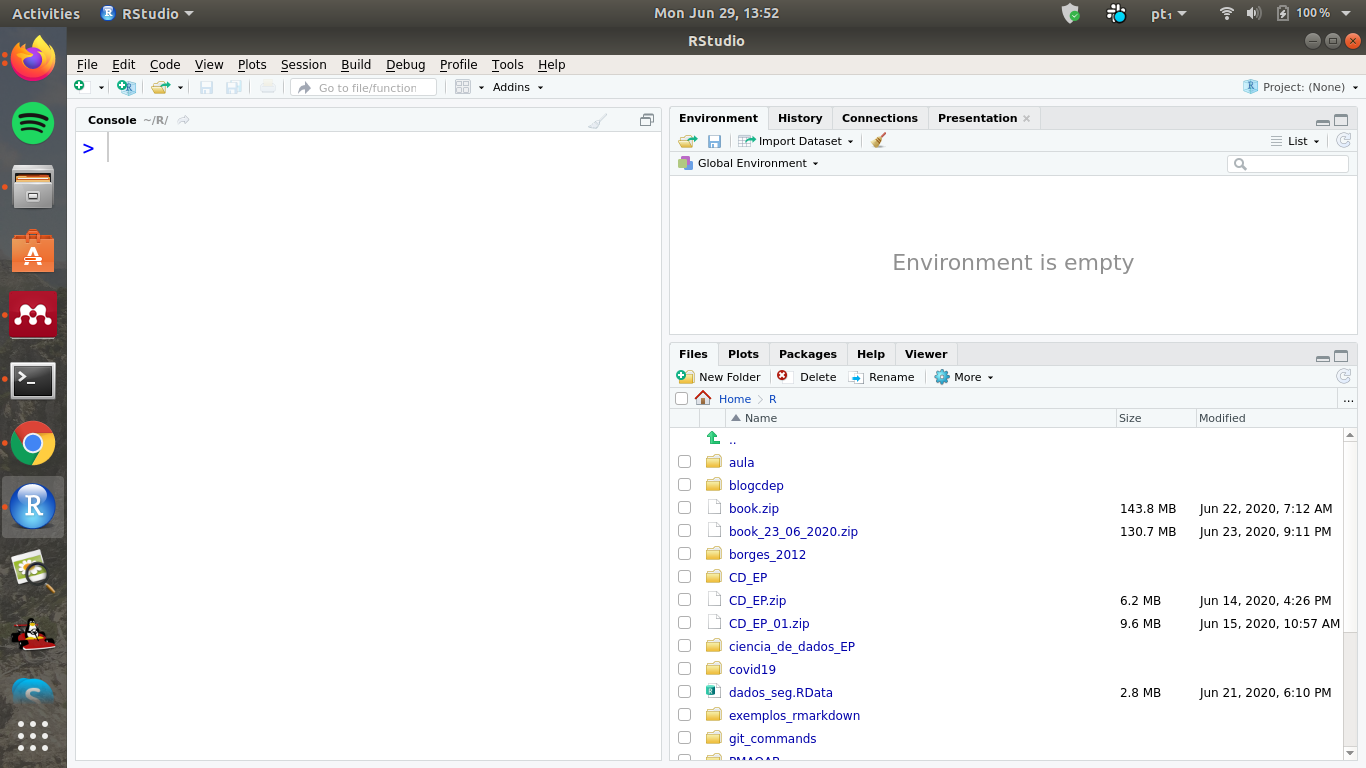
\includegraphics{fig/open_Rstudio.png}
\caption{Opção de instalação pelo modo gráfico}
\end{figure}

\begin{enumerate}
\def\labelenumi{\arabic{enumi}.}
\setcounter{enumi}{1}
\tightlist
\item
  Selecoine a aba de instalação \emph{Packages} e clique em
  \textbf{install},
\end{enumerate}

\begin{figure}
\centering
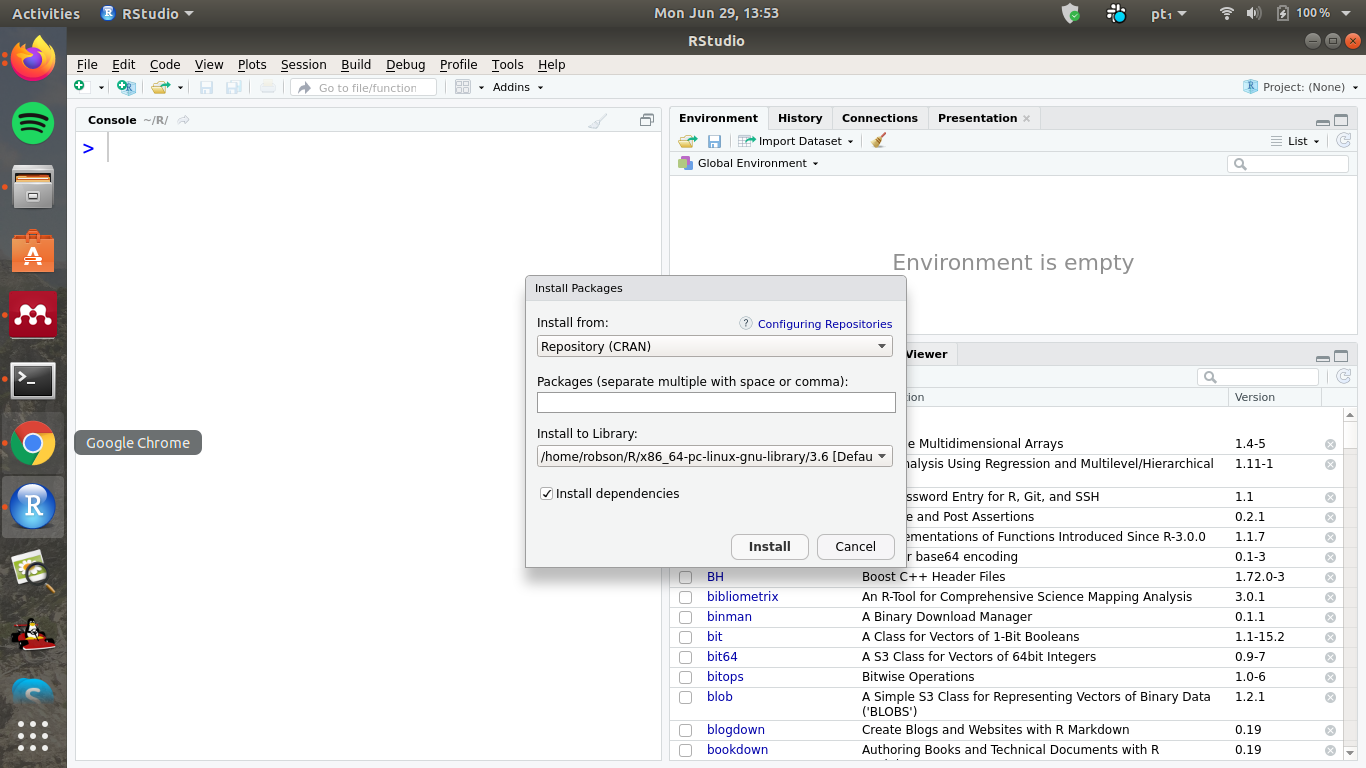
\includegraphics{fig/install_packages_rstudio_visual.png}
\caption{Selecoinar aba de instalação \emph{Packages - Click em
install}}
\end{figure}

\begin{enumerate}
\def\labelenumi{\arabic{enumi}.}
\setcounter{enumi}{2}
\tightlist
\item
  No ambiente de busca da interface instalação pesquise por
  \emph{bookdown}, selecione o pacote e clique em \emph{install},
\end{enumerate}

\begin{figure}
\centering
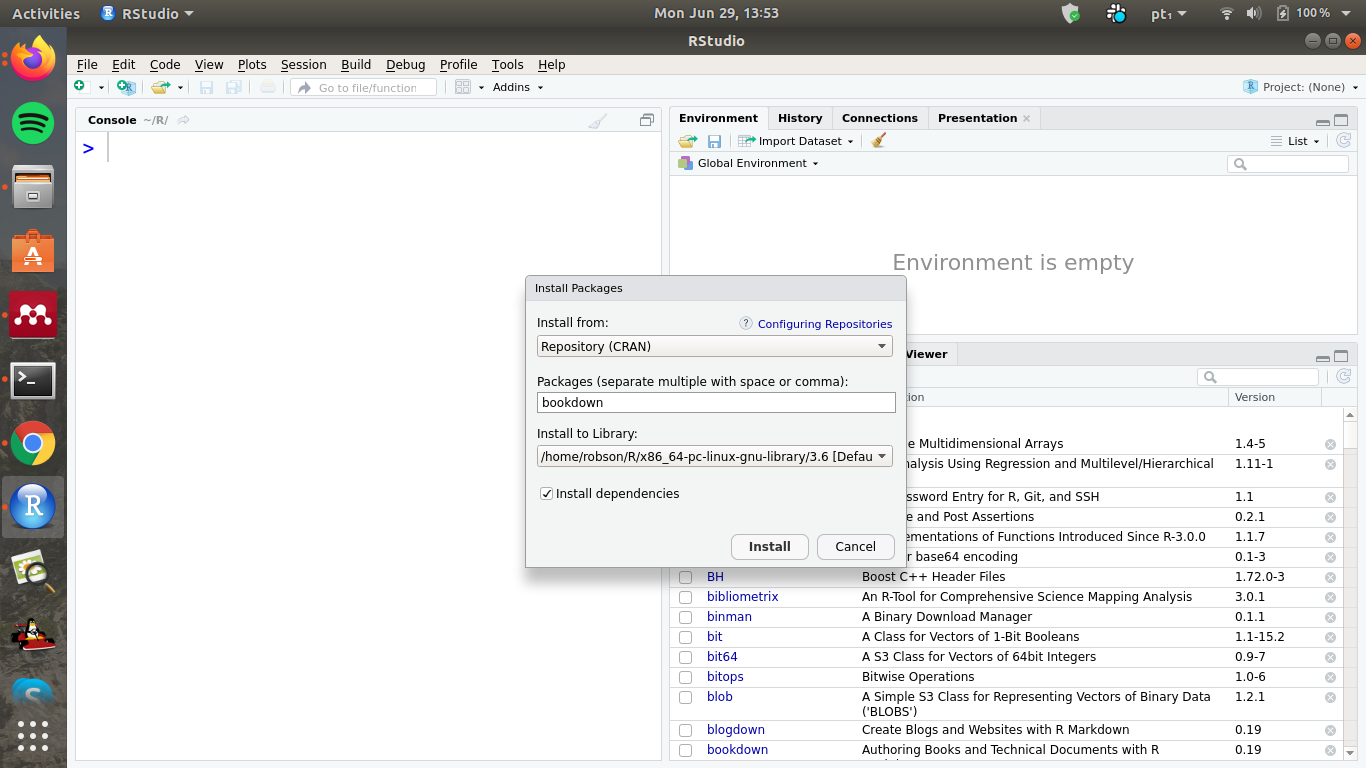
\includegraphics{fig/install_packages_rstudio_visual_bookdown.png}
\caption{\emph{Pesquisar por bookdown e clicar em install}}
\end{figure}

\begin{enumerate}
\def\labelenumi{\arabic{enumi}.}
\setcounter{enumi}{3}
\item
  Finalmente, o código será instalado,
  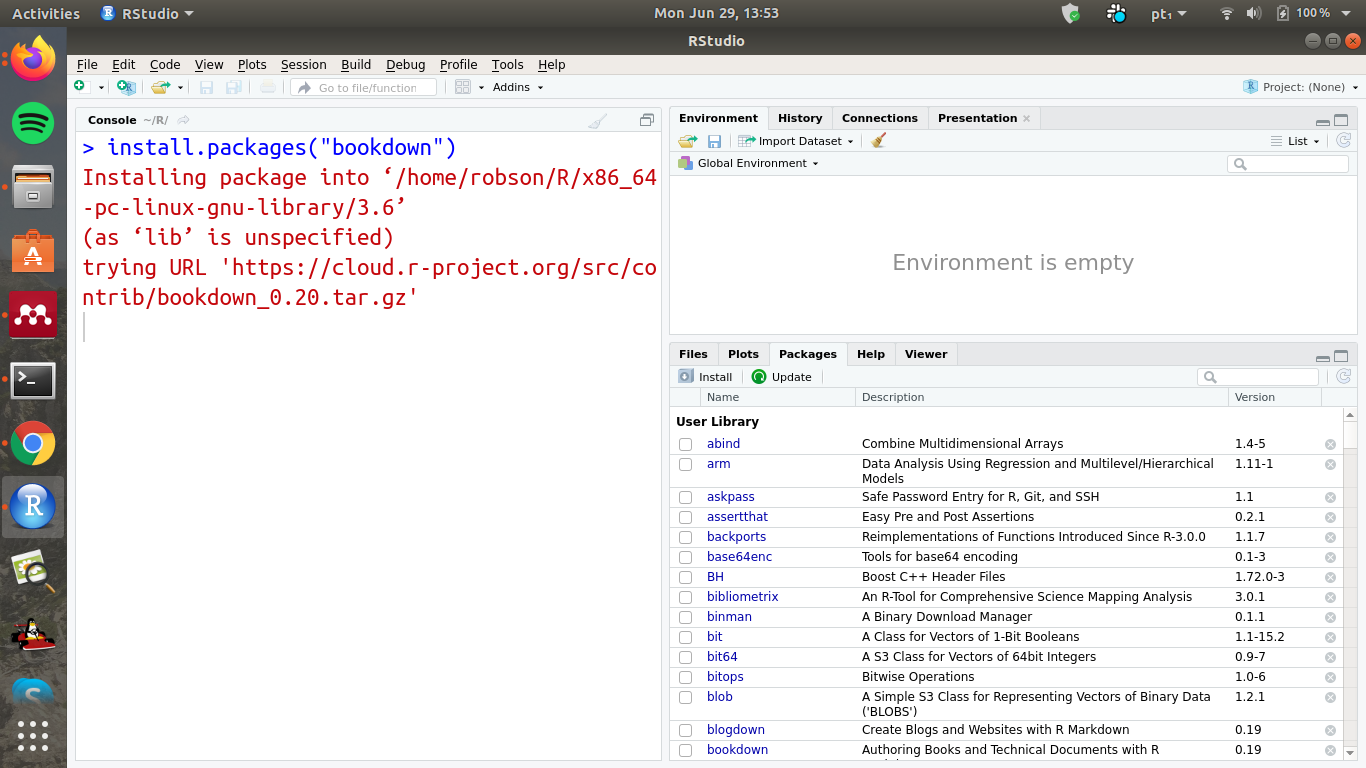
\includegraphics{fig/install_packages_rstudio_visual_bookdown_run.png}
\item
  Ainda é necessário carregá-lo na seção de uso, novamente na aba
  \emph{Packages} pesquise por \emph{bookdown} e selecione o pacote, o
  que será suficiente para carregá-lo,
\end{enumerate}

\begin{figure}
\centering
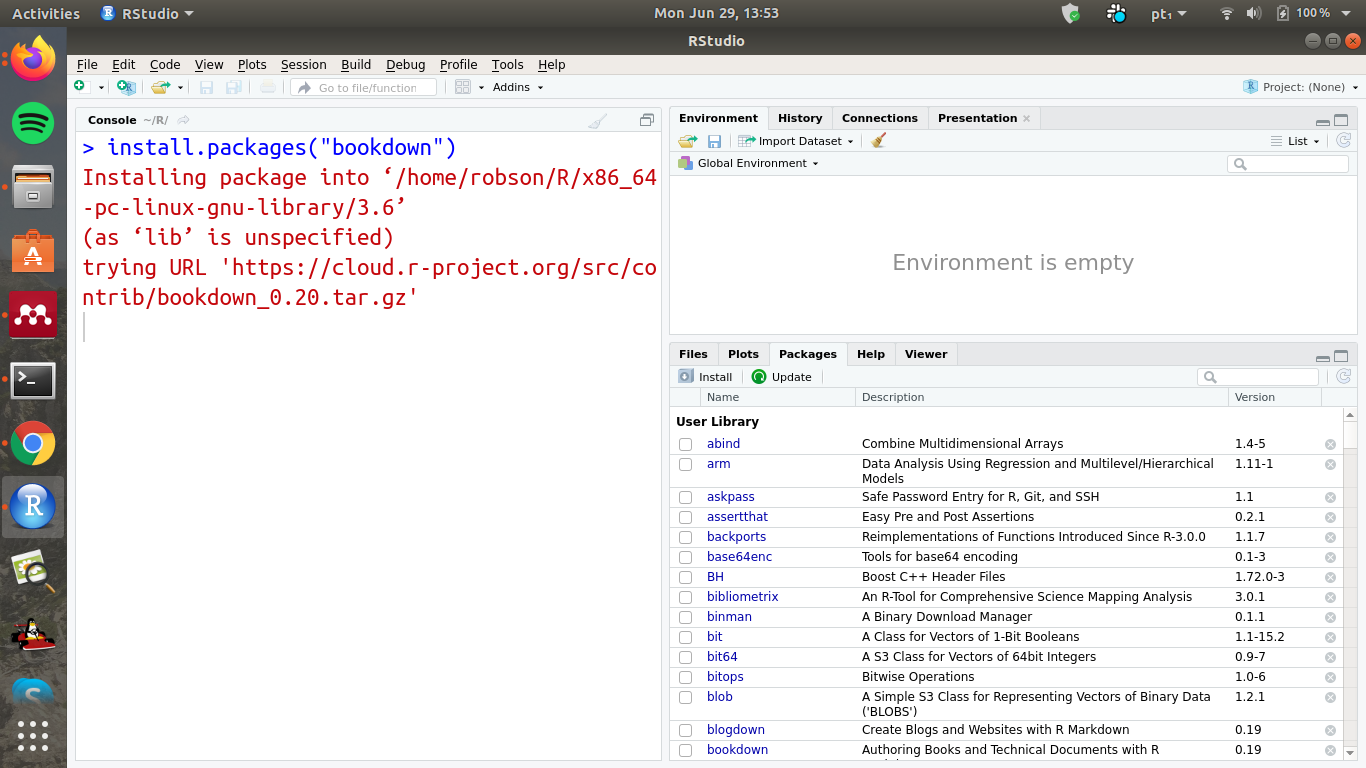
\includegraphics{fig/install_packages_rstudio_visual_bookdown_run.png}
\caption{Carregar a biblioteca bookdown na aba Package}
\end{figure}

\begin{Shaded}
\begin{Highlighting}[]
\KeywordTok{install.packages}\NormalTok{(}\StringTok{"bookdown"}\NormalTok{)}
\CommentTok{# or the development version}
\CommentTok{# devtools::install_github("rstudio/bookdown")}
\KeywordTok{library}\NormalTok{(}\StringTok{"bookdown"}\NormalTok{)}
\end{Highlighting}
\end{Shaded}

Deve-se lembrar que para cada arquivo \emph{.Rmd} só pode ter um
capítulo sendo definido pelo primeiro nível por \texttt{\#}.

Para compilar este exemplo para PDF, é necessário o pacote XeLaTeX. É
recomendável instalar o TinyTeX (que inclui o XeLaTeX):
\url{https://yihui.org/tinytex/}.

Nos próximos capítulos serão apresentados outros detalhes sobre
instalação e configuração.

\chapter{Introdução}\label{intro}

A primeira palavra que devemos pensar ao encarar um curso de ferramentas
de escrita de textos é \emph{oportunidade}.

Quando pensamos em texto simples e rápidos, podemos naturalmente usar
ferramentas como WYSIWYG (\emph{What You See Is What You Get}) como
\textbf{LibreOffice Writer} ou \textbf{Microsof Office Word}.
Entretanto, trabalhar com textos longos, como relatórios, trabalhos de
conclusão de curso (TCC), dissertações ou teses pode exigir recursos
mais avançados como LaTeX.

\section{Criação do projeto do
livro}\label{criauxe7uxe3o-do-projeto-do-livro}

Faremos uso mais uma vez de recursos gráficos da interface do
\emph{Rstudio} para a criação do projeto do livro. Este material foi
prepara utilizando a estrutura mínima disponibilizada pelo
\emph{template} do pacote \emph{bookdown}. As etapas a seguir serão o
suficiente para entender a criação e uso desse \emph{template}:

\begin{enumerate}
\def\labelenumi{\arabic{enumi}.}
\tightlist
\item
  Após a instalação e carregamento da biblioteca \emph{bookdown},
  podemos utilizar o \emph{template}, primeiro devemos clicar no canto
  superior direito em \emph{projetos} como:
\end{enumerate}

\begin{figure}
\centering
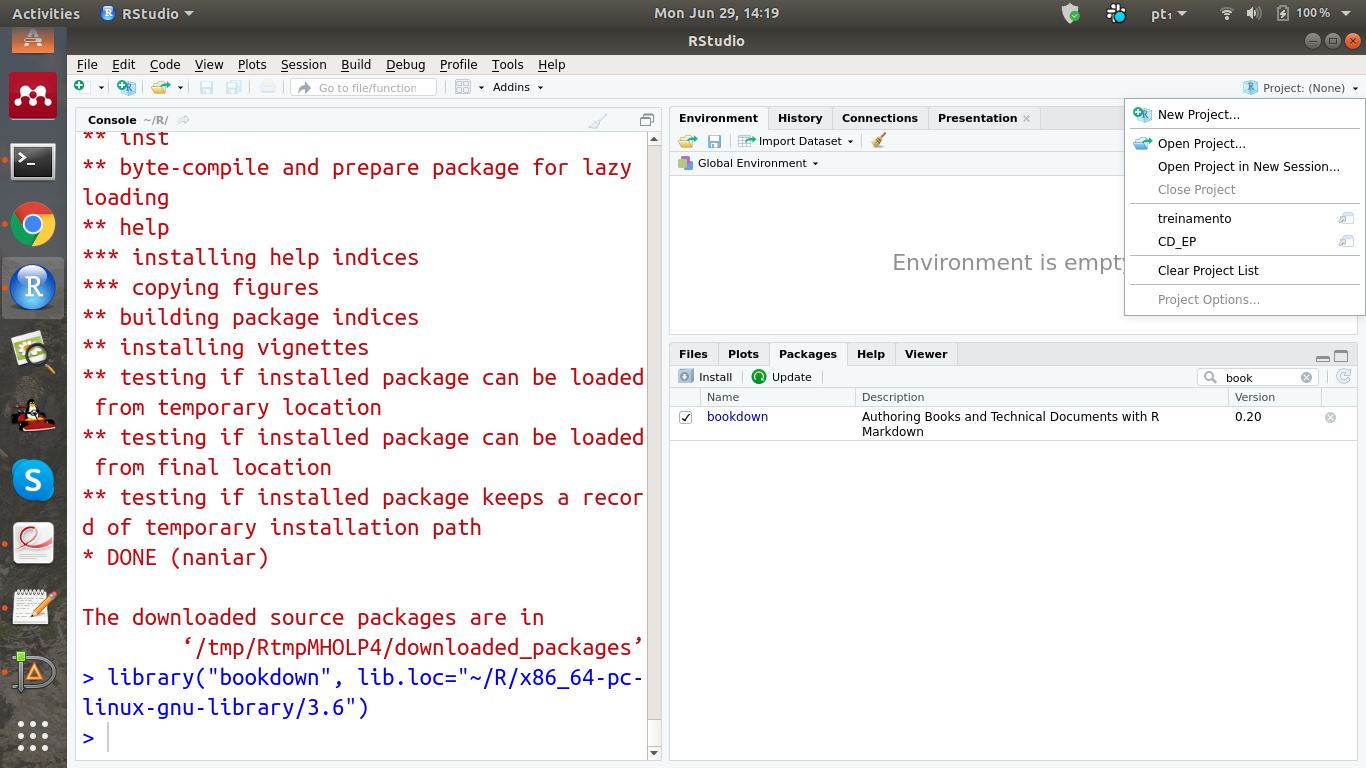
\includegraphics{fig/rstudio_select_new_Project.png}
\caption{Criação de um novo projeto de livro}
\end{figure}

\begin{enumerate}
\def\labelenumi{\arabic{enumi}.}
\setcounter{enumi}{1}
\tightlist
\item
  Em seguida, selecionar \emph{New Directory}:
\end{enumerate}

\begin{figure}
\centering
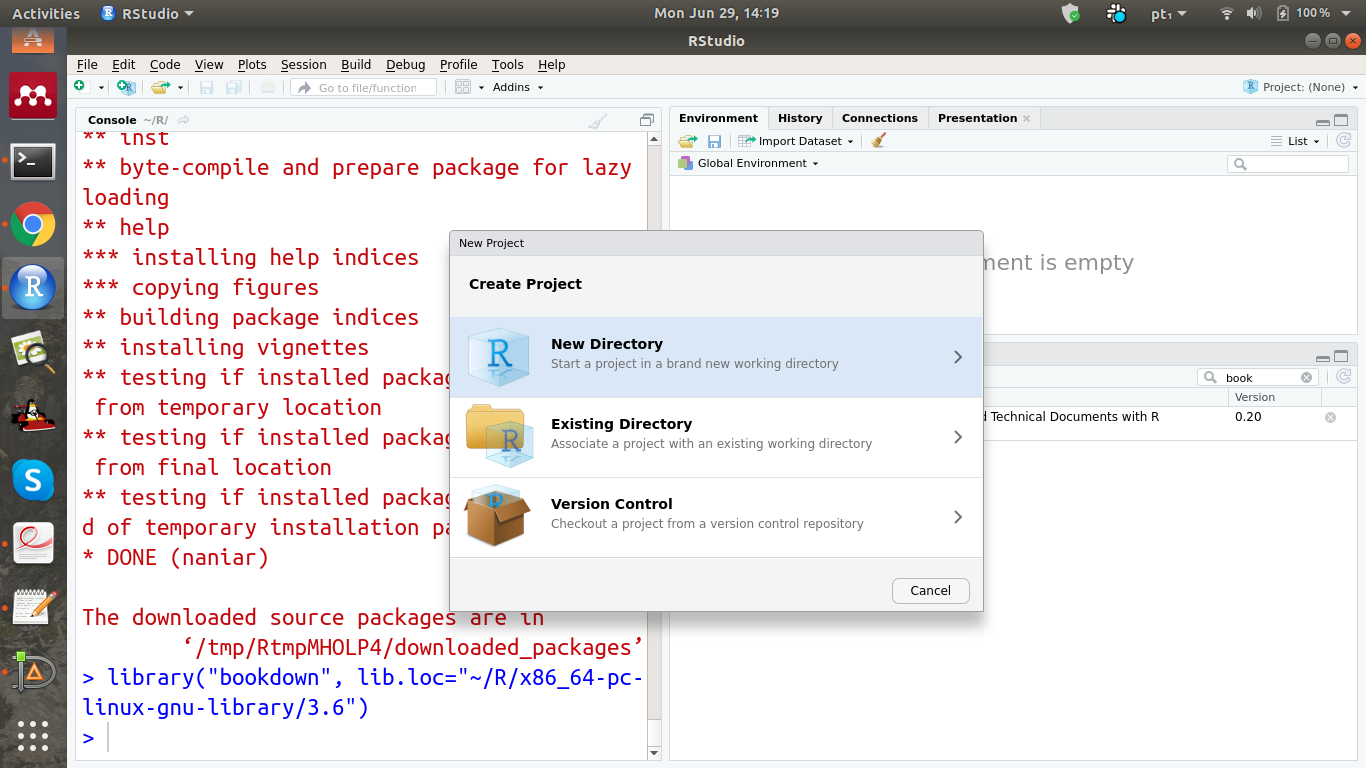
\includegraphics{fig/select_new_directory.png}
\caption{Selecionar a criação de um novo diretório}
\end{figure}

\begin{enumerate}
\def\labelenumi{\arabic{enumi}.}
\setcounter{enumi}{2}
\tightlist
\item
  Selecionar \emph{Book Project with bookdown}
\end{enumerate}

\begin{figure}
\centering
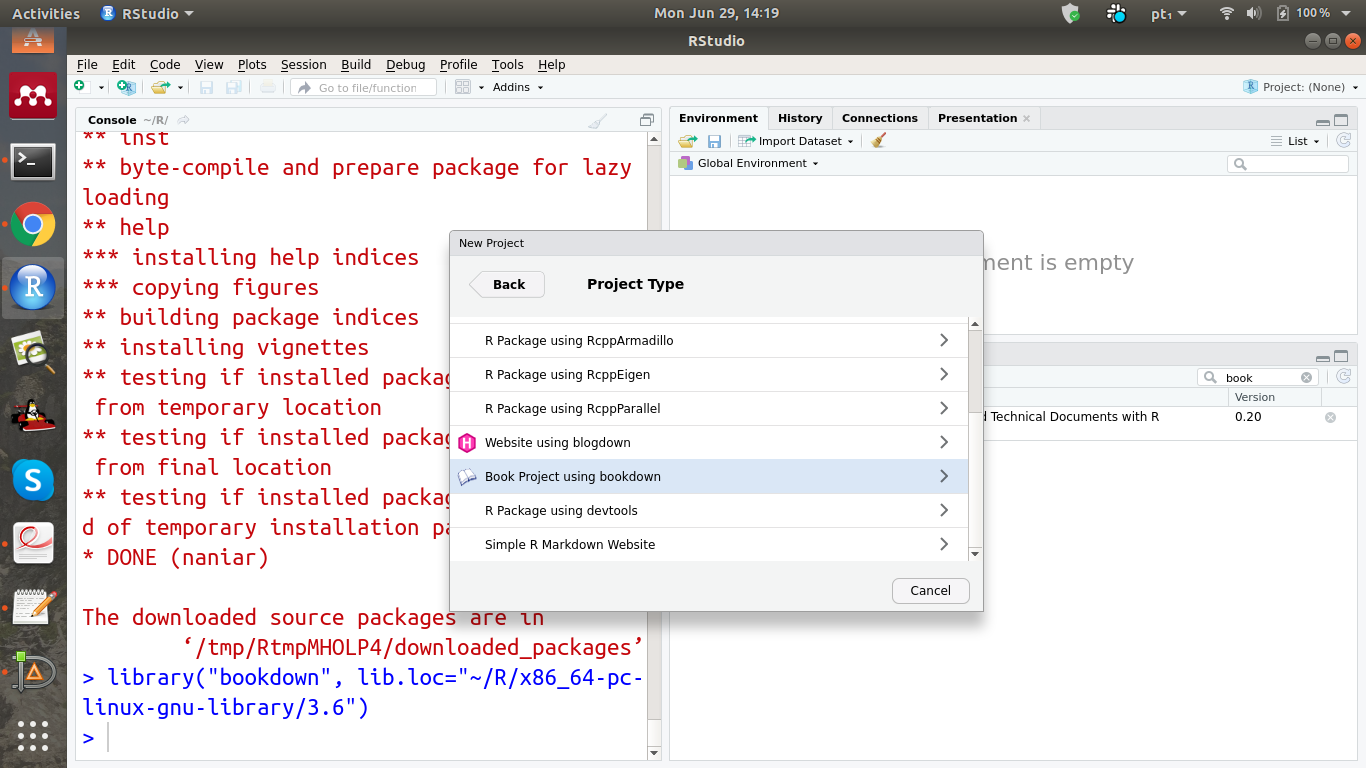
\includegraphics{fig/select_Book_Project_with_bookdown.png}
\caption{Seleção da opção de projeto de livro com pacote bookdown}
\end{figure}

\begin{enumerate}
\def\labelenumi{\arabic{enumi}.}
\setcounter{enumi}{3}
\tightlist
\item
  Em seguida o template com a versão mínima será disponibilizado por
  meio de uma pasta com o nome escolhido na etapa anterior.
\end{enumerate}

\begin{figure}
\centering
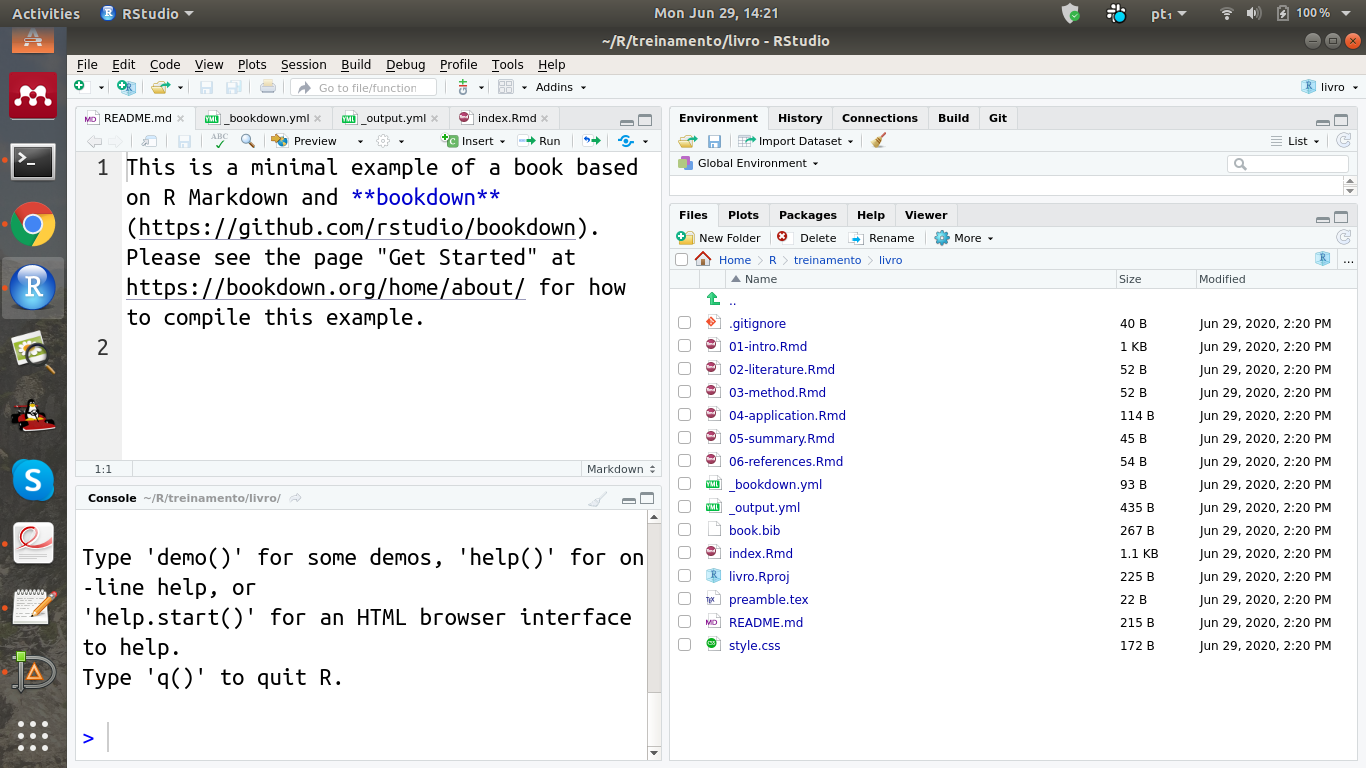
\includegraphics{fig/outra.png}
\caption{Seleção da opção de projeto de livro com pacote bookdown}
\end{figure}

Na lista apresentada acima são identificados arquivos com as seguintes
extensões:

\begin{itemize}
\tightlist
\item
  \textbf{.Rmd}
\item
  \textbf{.bib}
\item
  \textbf{.yml}
\item
  \textbf{.tex}
\item
  \textbf{.css}
\end{itemize}

Aqueles arquivos cuja a extensão é \emph{.Rmd} são utilizados para a
escrita dos conteúdos do livro em R Markdown. Entretanto, entre eles há
um especial, \emph{index.Rmd}, que constrói a página principal, por meio
de comandos \textbf{yml}. Algumas configurações são reservadas em dois
arquivos com extensão \textbf{.yml}. Sendo o arquivo \_bookdown.yml para
configurações gerais que serão úteis para quaisquer tipo de documento de
saída, por exemplo, a definição se o título de cada capítulo será
chamado de \textbf{Chapter } ou \textbf{Capítulo }, especialmente para
este treinamento fizemos esta alteração. Enquanto que para o arquivo
*\_output.yml* são apresentadas configurações especiais para cada tipo
de saída, como \emph{bookdown::gitbook}, \emph{bookdown::pdf\_book:} ou
\emph{bookdown::epub\_book:}. Especialmente para o caso do
\emph{gitbook} é necessário a existência do arquivo \emph{style.css}
para algumas configurações. Já o arquivo \emph{book.bib} é uma estrutura
especial do pacote \emph{bibtex} do LaTeX e contem as informações de
artigos que serão citados.

\chapter{Literatura e bibtex}\label{literatura-e-bibtex}

O foco deste capítulo está numa das principais potencialidades do LaTeX
utilizas pelo R Markdown a capacidade de citar os documentos
adequadamente organizados num arquivo \emph{.bib}, especialmente neste
exemplo aproveitamos o arquivo gerado pela estrutura mínima
\emph{bookdown}.

Para esta etapa aproveitaremos como exemplo os artigos do projeto
organizados na plataforma Mendeley, seguindo os seguintes passos:

\begin{enumerate}
\def\labelenumi{\arabic{enumi}.}
\tightlist
\item
  Abrir Medeley Desktop;
\item
  Abrir pasta do grupo nomeada por CDnaEP;
\item
  Selecionar os artigos que pretende citar no seu documento;
\item
  Clicar com o botão direito do mouse, selecionar \emph{Copy as} e em
  seguida \emph{BibTex entry}.
\item
  Abrir o arquivo \emph{book.bib} e colar os metadados dos artigos na
  última linha do arquivo depois da última chave \textbf{\}}.
\item
  Em seguida, salve e feche o arquivo \emph{book.bib}.
\end{enumerate}

As figuras a seguir estão de acordo com a sequência acima apresentada:

\begin{figure}
\centering
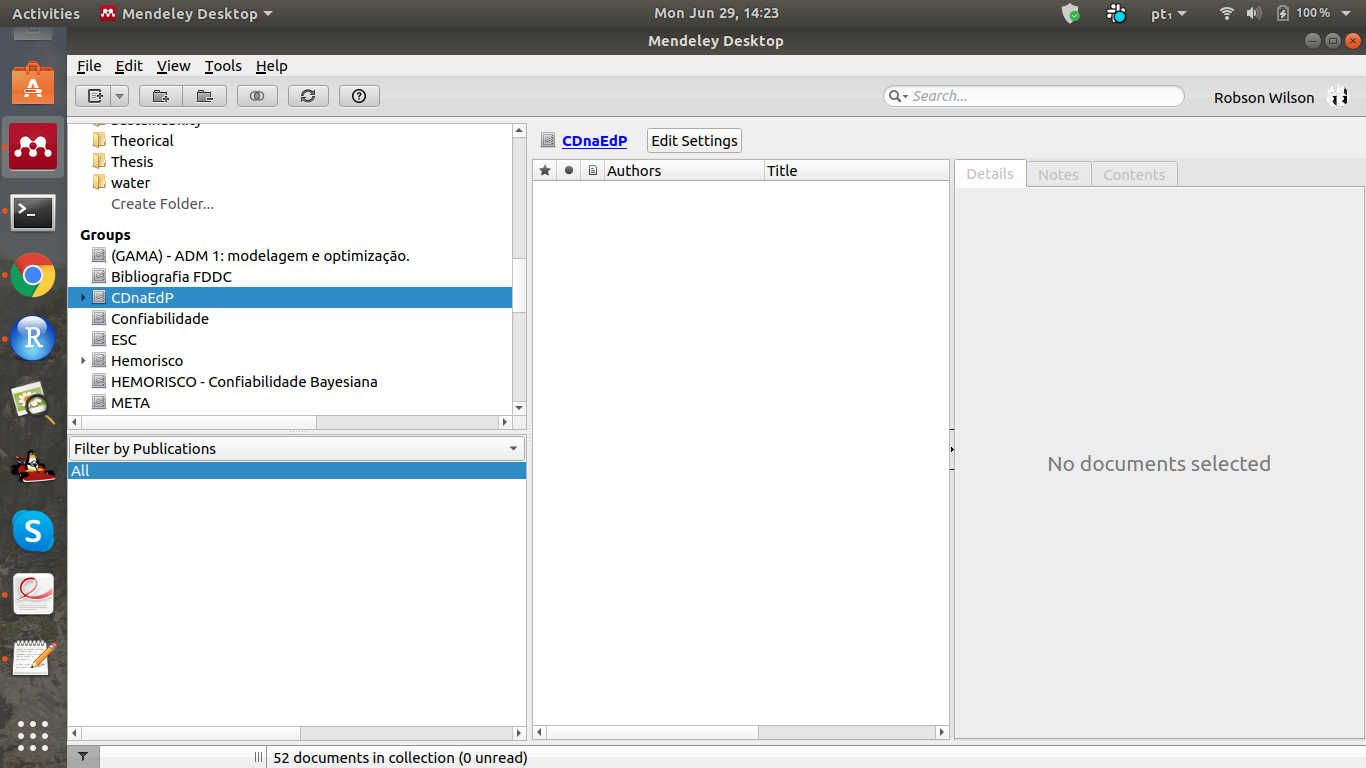
\includegraphics{fig/open_mendeley.png}
\caption{Abrir Medeley Desktop e selecionar pasta CDna EP}
\end{figure}

\begin{figure}
\centering
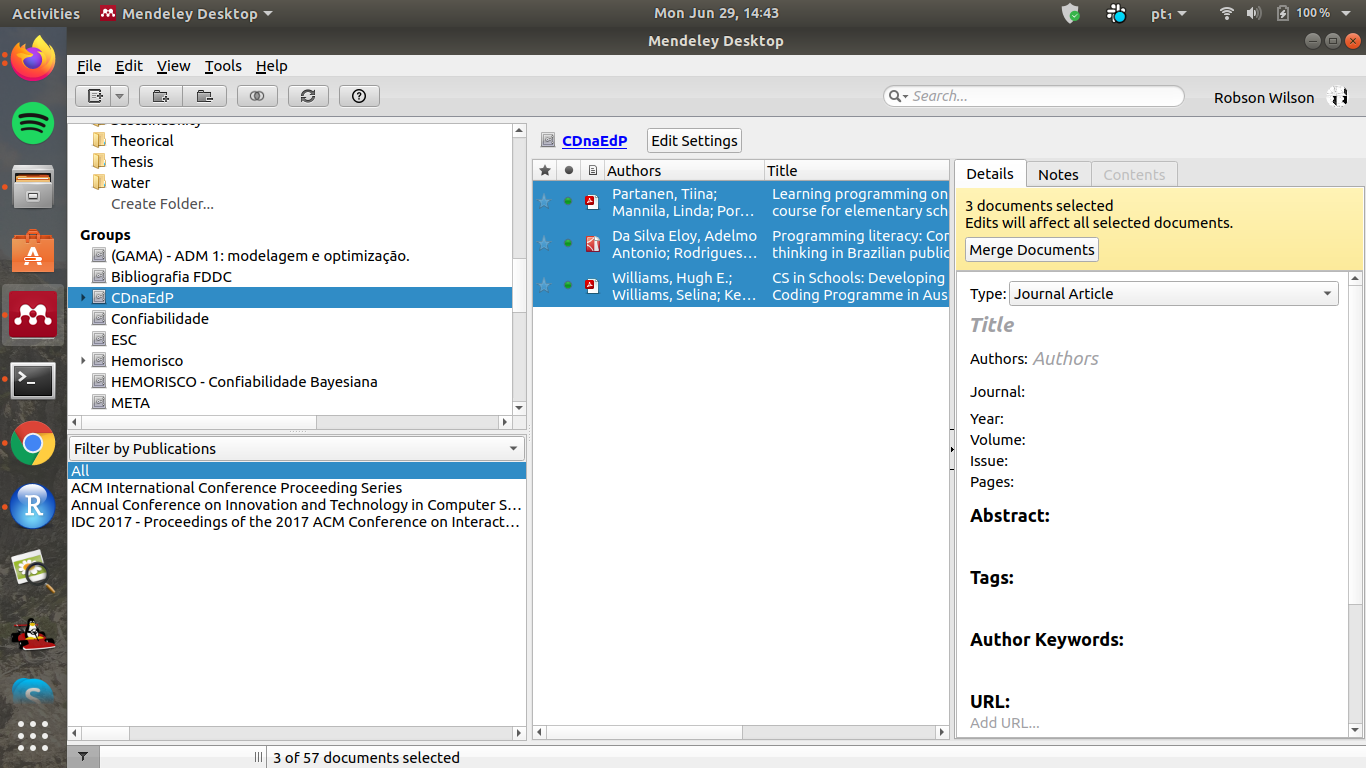
\includegraphics{fig/mendeley_select_CDnaEP_paper_list.png}
\caption{Selecionar artigos para citação}
\end{figure}

\begin{figure}
\centering
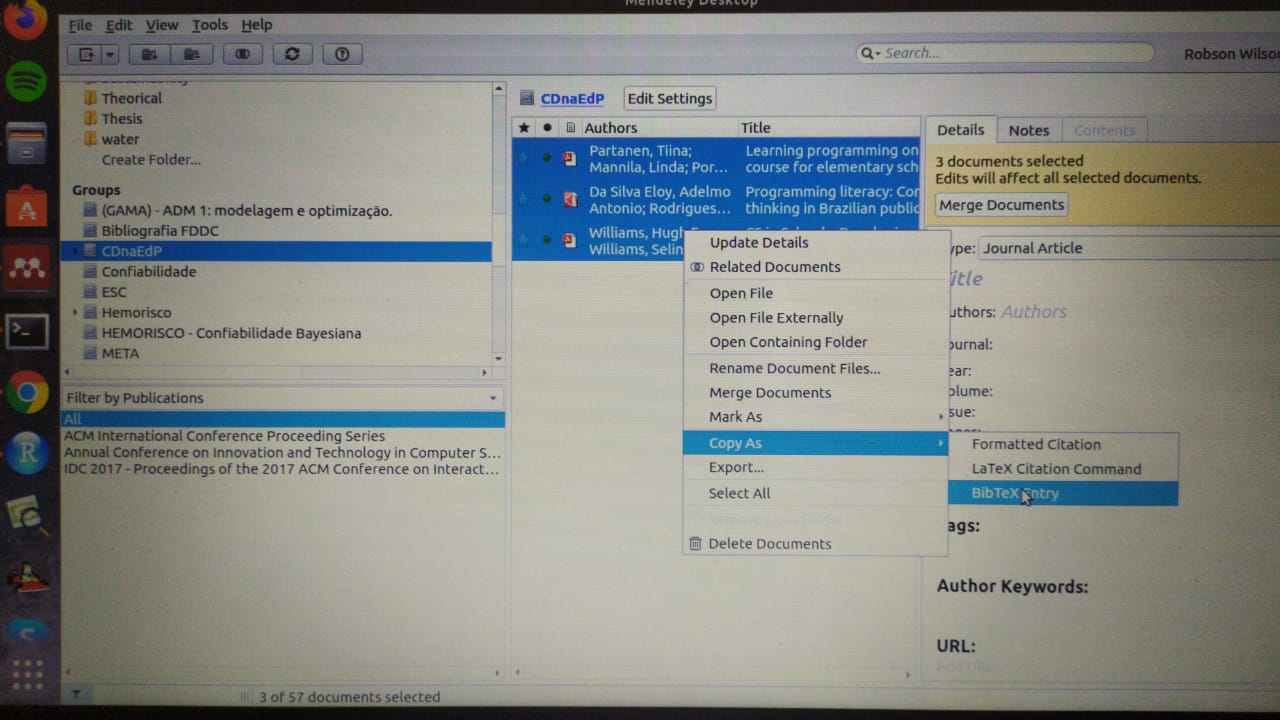
\includegraphics{fig/mendeley_copy_bibtex_entry.jpeg}
\caption{Copiar metadados no formato de entrada do bibtex}
\end{figure}

Uma informação importante para quem ainda não é familiarizado com LaTeX
é o fato da primeira informação dos metados de um artigo dentro do
arquivo \emph{.bib} ser a \emph{label}, a informação que será usada para
citações ao longo do documento.

\begin{figure}
\centering
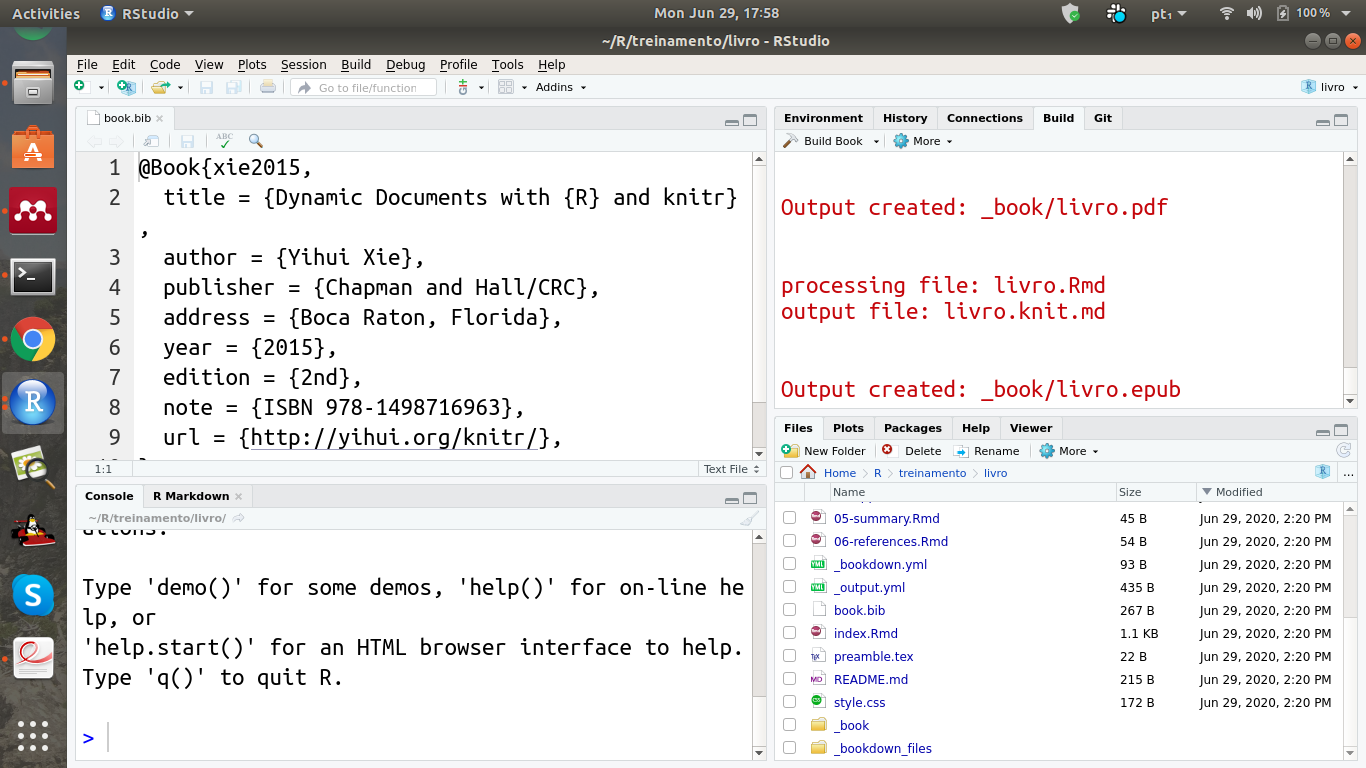
\includegraphics{fig/rstudio_open_bookbib_first.png}
\caption{Identificação da \emph{label} do livro do (\citep{xie2015})}
\end{figure}

\begin{figure}
\centering
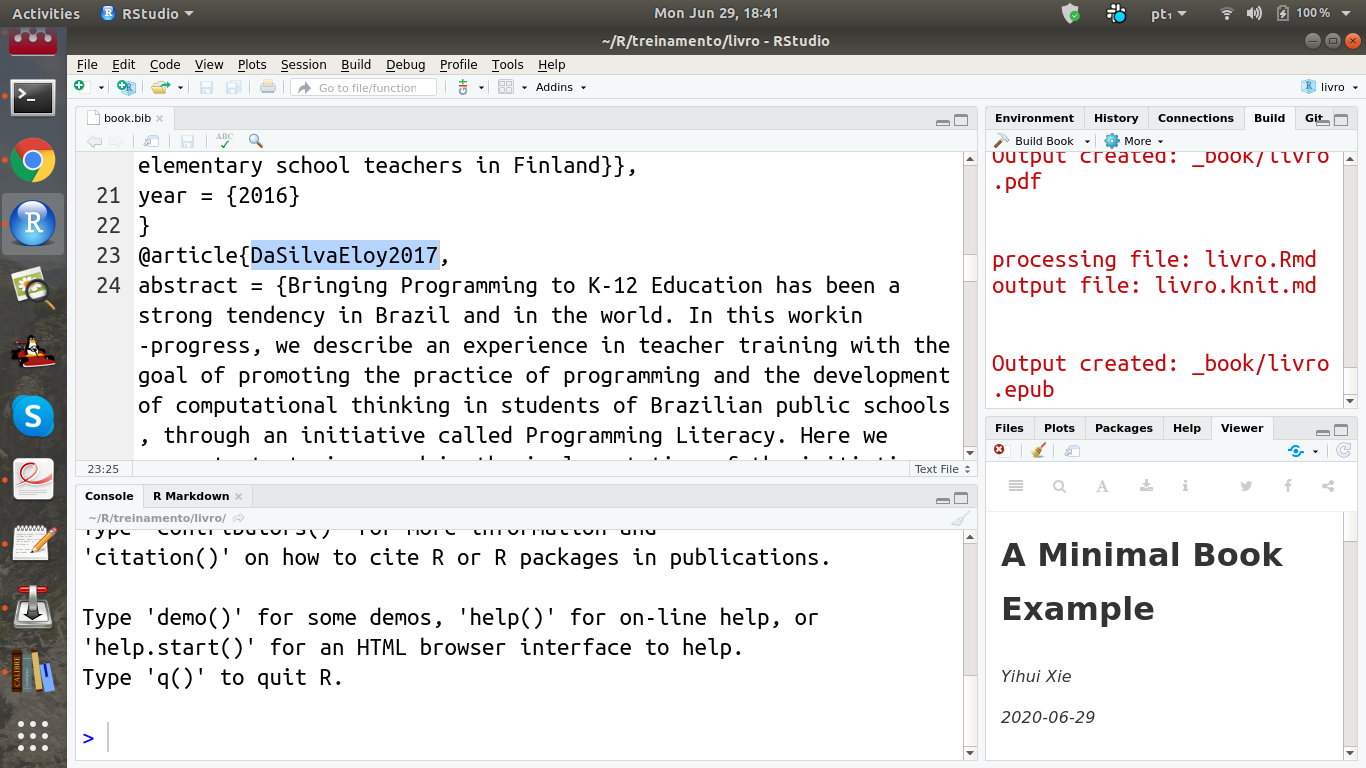
\includegraphics{fig/rstudio_open_bookbib_second.png}
\caption{Identificação da \emph{label} de cada artigo
(\citep{DaSilvaEloy2017})}
\end{figure}

\begin{figure}
\centering
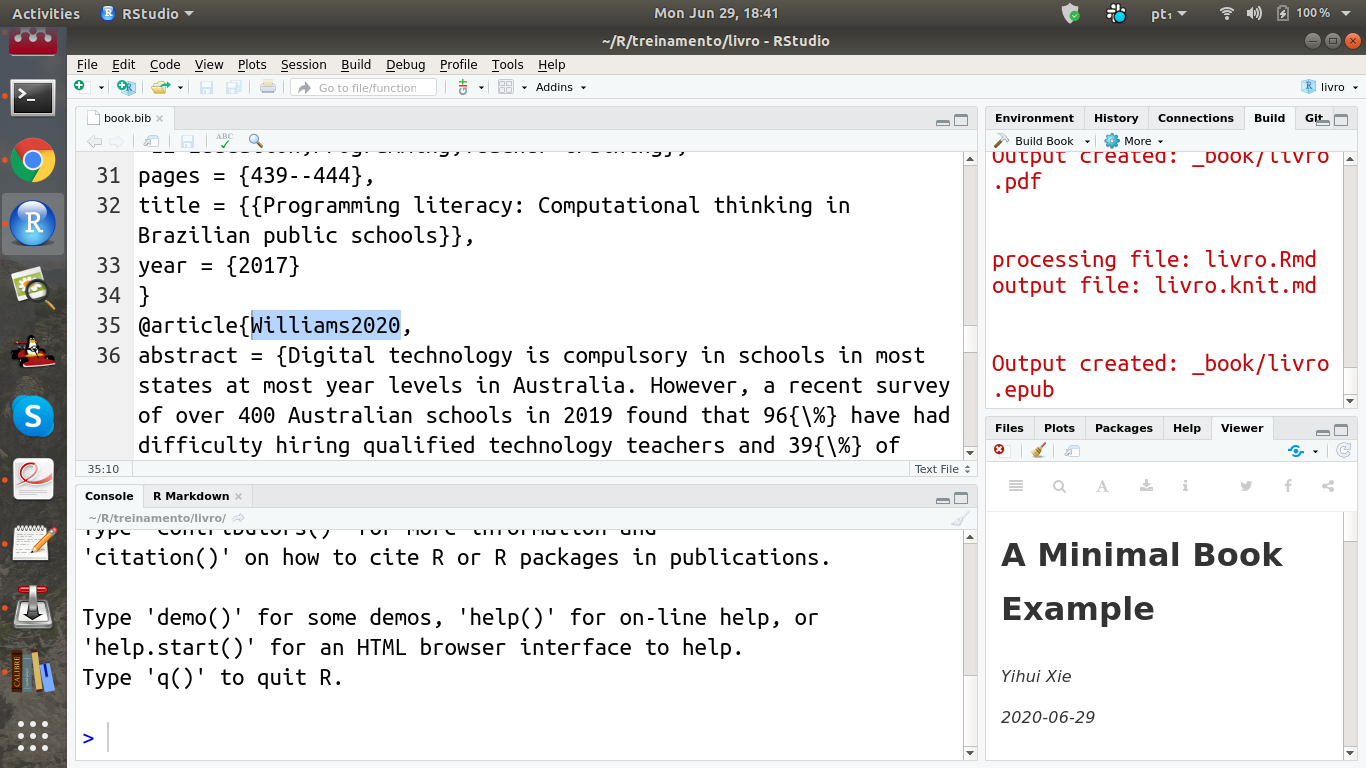
\includegraphics{fig/rstudio_open_bookbib_third.png}
\caption{Identificação da \emph{label} de cada artigo
(\citep{Williams2020})}
\end{figure}

Nas subseções a seguir mostramos como citar alguns desses trabalhos.

\section{Exemplo de citação
simples}\label{exemplo-de-citauxe7uxe3o-simples}

Vamos considerar a citação do artigo \citep{Partanen2016}.

\section{Citações de dois ou mais
artigos}\label{citauxe7uxf5es-de-dois-ou-mais-artigos}

Agora incluiremos mais duas citações
\citep[\citet{Williams2020}]{DaSilvaEloy2017}.

\chapter{Métodos}\label{metodos}

Alguns detalhes como colocar uma \texttt{\{\#label\}} para se referir de
forma automática a uma seção ou capítulo é feito de maneira de forma
simples. Depois de incluída a \emph{label} podemos citar a referida
seção ou capítulo do comando pelo comando \ref{intro}.

Figuras e tabelas com títulos podem ser inseridas pelos respectivos
ambientes \texttt{figure} e \texttt{table}.

\begin{Shaded}
\begin{Highlighting}[]
\KeywordTok{par}\NormalTok{(}\DataTypeTok{mar =} \KeywordTok{c}\NormalTok{(}\DecValTok{4}\NormalTok{, }\DecValTok{4}\NormalTok{, .}\DecValTok{1}\NormalTok{, .}\DecValTok{1}\NormalTok{))}
\KeywordTok{plot}\NormalTok{(pressure, }\DataTypeTok{type =} \StringTok{'b'}\NormalTok{, }\DataTypeTok{pch =} \DecValTok{19}\NormalTok{)}
\end{Highlighting}
\end{Shaded}

\begin{figure}

{\centering 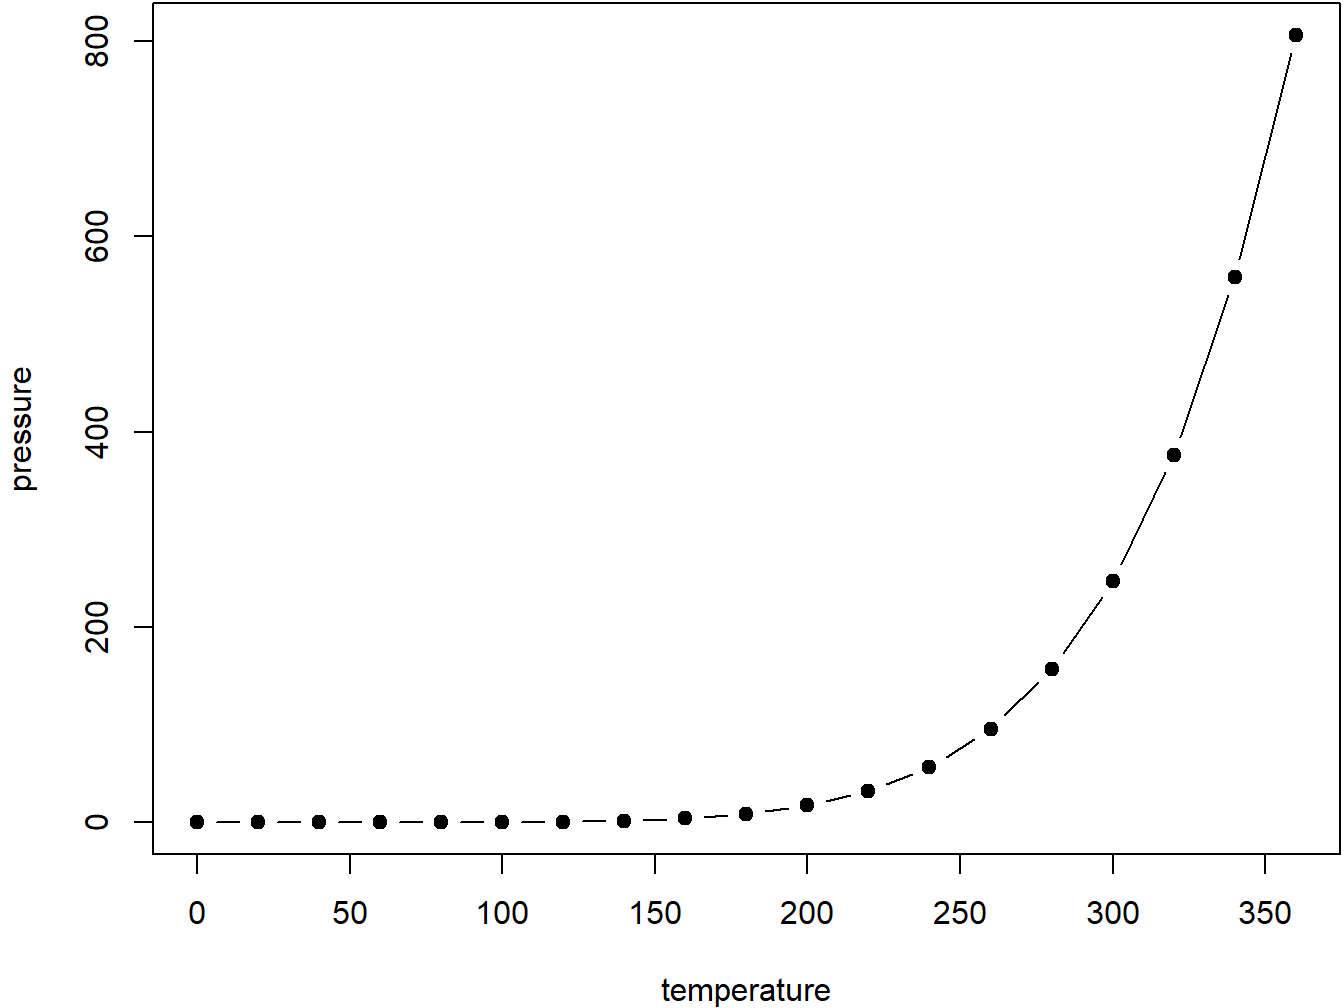
\includegraphics[width=0.8\linewidth]{livro_files/figure-latex/nice-fig-1} 

}

\caption{Comportamento da pressão.}\label{fig:nice-fig}
\end{figure}

A forma de se referir pela figura é através do \emph{label} do
\emph{chunck} no qual foi produzida com prefixo \texttt{fig:}, e.g., ver
Figura \ref{fig:nice-fig}. De forma similar, você pode se referir a
tabelas geradas por \texttt{knitr::kable()}, e.g., ver Tabela
\ref{tab:nice-tab}.

\begin{Shaded}
\begin{Highlighting}[]
\NormalTok{knitr}\OperatorTok{::}\KeywordTok{kable}\NormalTok{(}
  \KeywordTok{head}\NormalTok{(iris, }\DecValTok{20}\NormalTok{), }\DataTypeTok{caption =} \StringTok{'Here is a nice table!'}\NormalTok{,}
  \DataTypeTok{booktabs =} \OtherTok{TRUE}
\NormalTok{)}
\end{Highlighting}
\end{Shaded}

\begin{table}

\caption{\label{tab:nice-tab}Here is a nice table!}
\centering
\begin{tabular}[t]{rrrrl}
\toprule
Sepal.Length & Sepal.Width & Petal.Length & Petal.Width & Species\\
\midrule
5.1 & 3.5 & 1.4 & 0.2 & setosa\\
4.9 & 3.0 & 1.4 & 0.2 & setosa\\
4.7 & 3.2 & 1.3 & 0.2 & setosa\\
4.6 & 3.1 & 1.5 & 0.2 & setosa\\
5.0 & 3.6 & 1.4 & 0.2 & setosa\\
\addlinespace
5.4 & 3.9 & 1.7 & 0.4 & setosa\\
4.6 & 3.4 & 1.4 & 0.3 & setosa\\
5.0 & 3.4 & 1.5 & 0.2 & setosa\\
4.4 & 2.9 & 1.4 & 0.2 & setosa\\
4.9 & 3.1 & 1.5 & 0.1 & setosa\\
\addlinespace
5.4 & 3.7 & 1.5 & 0.2 & setosa\\
4.8 & 3.4 & 1.6 & 0.2 & setosa\\
4.8 & 3.0 & 1.4 & 0.1 & setosa\\
4.3 & 3.0 & 1.1 & 0.1 & setosa\\
5.8 & 4.0 & 1.2 & 0.2 & setosa\\
\addlinespace
5.7 & 4.4 & 1.5 & 0.4 & setosa\\
5.4 & 3.9 & 1.3 & 0.4 & setosa\\
5.1 & 3.5 & 1.4 & 0.3 & setosa\\
5.7 & 3.8 & 1.7 & 0.3 & setosa\\
5.1 & 3.8 & 1.5 & 0.3 & setosa\\
\bottomrule
\end{tabular}
\end{table}

Você pode fazer citações, nós estamos usando o pacote \textbf{bookdown}
\citep{R-bookdown} neste livro de amostra, o qual foi compilado por R
Markdown e \textbf{knitr} \citep{xie2015}.

\section{Analisando o uso de chunks}\label{analisando-o-uso-de-chunks}

\subsection{Chunk - Condição
padrão}\label{chunk---condiuxe7uxe3o-padruxe3o}

A condição \emph{default} do \emph{rmarkdown} é a execução do código,
apresentação do código e do resultado do processamento.

Criaremos inicialmente uma função no R markdown:

\begin{Shaded}
\begin{Highlighting}[]
\NormalTok{exps<-}\ControlFlowTok{function}\NormalTok{(t,l,k,c)\{}
\NormalTok{ exps <-}\StringTok{ }\KeywordTok{exp}\NormalTok{(}\OperatorTok{-}\NormalTok{l}\OperatorTok{*}\NormalTok{(k}\OperatorTok{**}\NormalTok{(}\DecValTok{1}\OperatorTok{-}\NormalTok{c))}\OperatorTok{*}\NormalTok{t)}
\NormalTok{\}}
\end{Highlighting}
\end{Shaded}

.

Em seguida, aplicaremos esta mesma função em um \emph{chunck}:

\begin{Shaded}
\begin{Highlighting}[]
\NormalTok{t<-}\KeywordTok{seq}\NormalTok{(}\DecValTok{1}\NormalTok{,}\DecValTok{10}\NormalTok{,}\FloatTok{0.1}\NormalTok{)}
\NormalTok{l<-}\FloatTok{1e-5}
\NormalTok{c<-}\FloatTok{0.95}
\NormalTok{k<-}\DecValTok{350}
\NormalTok{Rb <-}\StringTok{ }\KeywordTok{exps}\NormalTok{(t,l,k,c)}
\KeywordTok{plot}\NormalTok{(t,Rb)}
\end{Highlighting}
\end{Shaded}

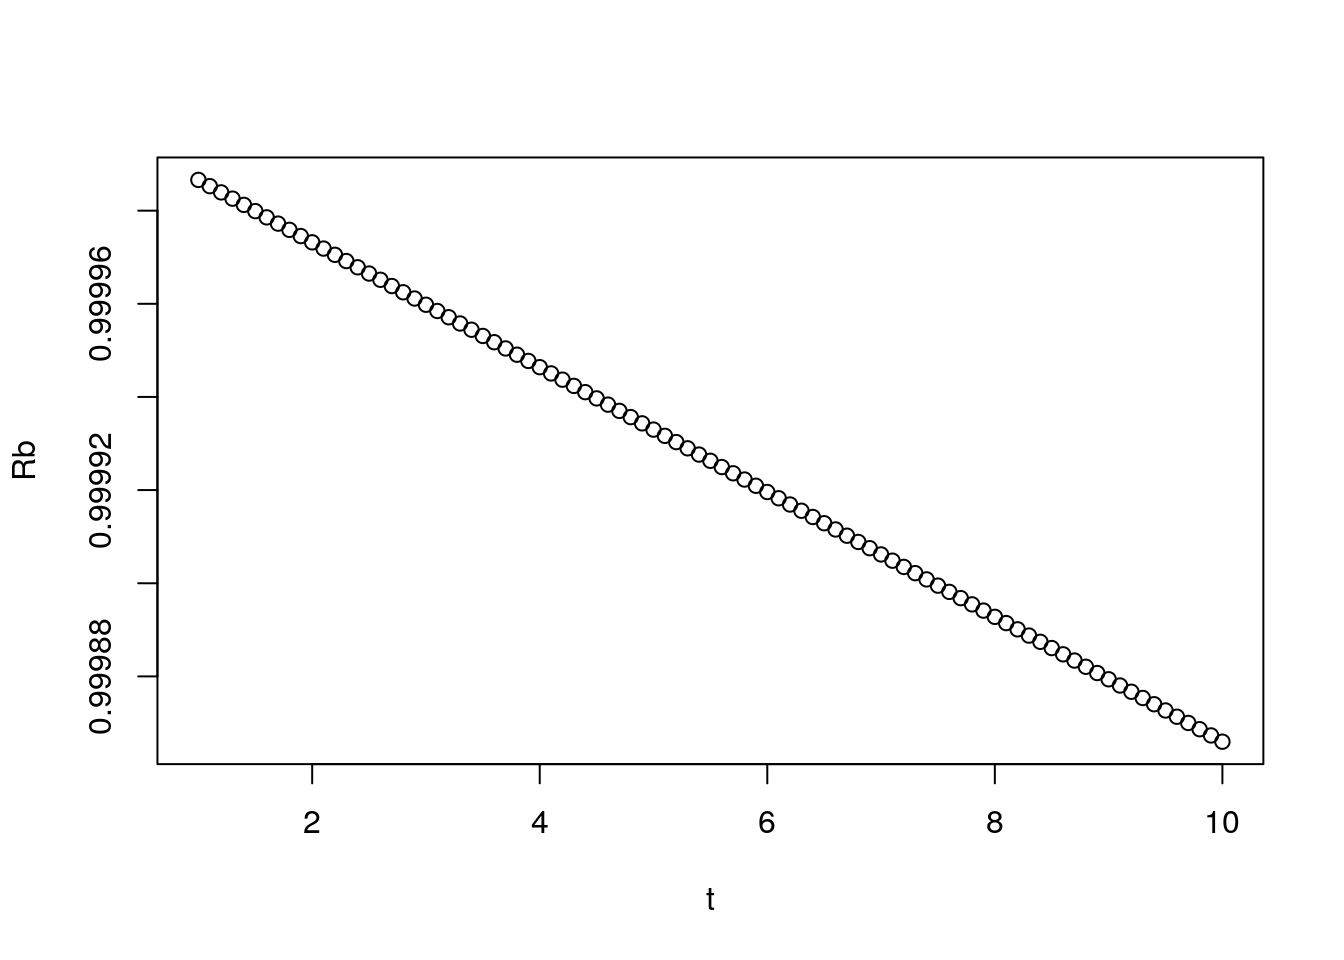
\includegraphics{livro_files/figure-latex/unnamed-chunk-6-1.pdf}

Como observado acima, os códigos e resultados são apresentados.

\subsection{Aparecer código e sem
executá-lo}\label{aparecer-cuxf3digo-e-sem-executuxe1-lo}

Nesta seção utilizaremos a opção \textbf{eval=FALSE}, assim o código
será apresentado sem executá-lo, ou seja, não haverá resultados.

\begin{Shaded}
\begin{Highlighting}[]
\NormalTok{exps<-}\ControlFlowTok{function}\NormalTok{(t,l,k,c)\{}
\NormalTok{ exps <-}\StringTok{ }\KeywordTok{exp}\NormalTok{(}\OperatorTok{-}\NormalTok{l}\OperatorTok{*}\NormalTok{(k}\OperatorTok{**}\NormalTok{(}\DecValTok{1}\OperatorTok{-}\NormalTok{c))}\OperatorTok{*}\NormalTok{t)}
\NormalTok{\}}
\end{Highlighting}
\end{Shaded}

.

Em seguida, aplicaremos esta mesma função em um \emph{chunck}:

\begin{Shaded}
\begin{Highlighting}[]
\NormalTok{t<-}\KeywordTok{seq}\NormalTok{(}\DecValTok{1}\NormalTok{,}\DecValTok{10}\NormalTok{,}\FloatTok{0.1}\NormalTok{)}
\NormalTok{l<-}\FloatTok{1e-5}
\NormalTok{c<-}\FloatTok{0.95}
\NormalTok{k<-}\DecValTok{350}
\NormalTok{Rb <-}\StringTok{ }\KeywordTok{exps}\NormalTok{(t,l,k,c)}
\KeywordTok{plot}\NormalTok{(t,Rb)}
\end{Highlighting}
\end{Shaded}

\subsection{Executar código sem
apresentá-lo}\label{executar-cuxf3digo-sem-apresentuxe1-lo}

Nesta seção utilizaremos a opção \textbf{echo=FALSE}, assim o código
será apresentado sem executá-lo, ou seja, não haverá resultados.

.

Em seguida, aplicaremos esta mesma função em um \emph{chunck}:

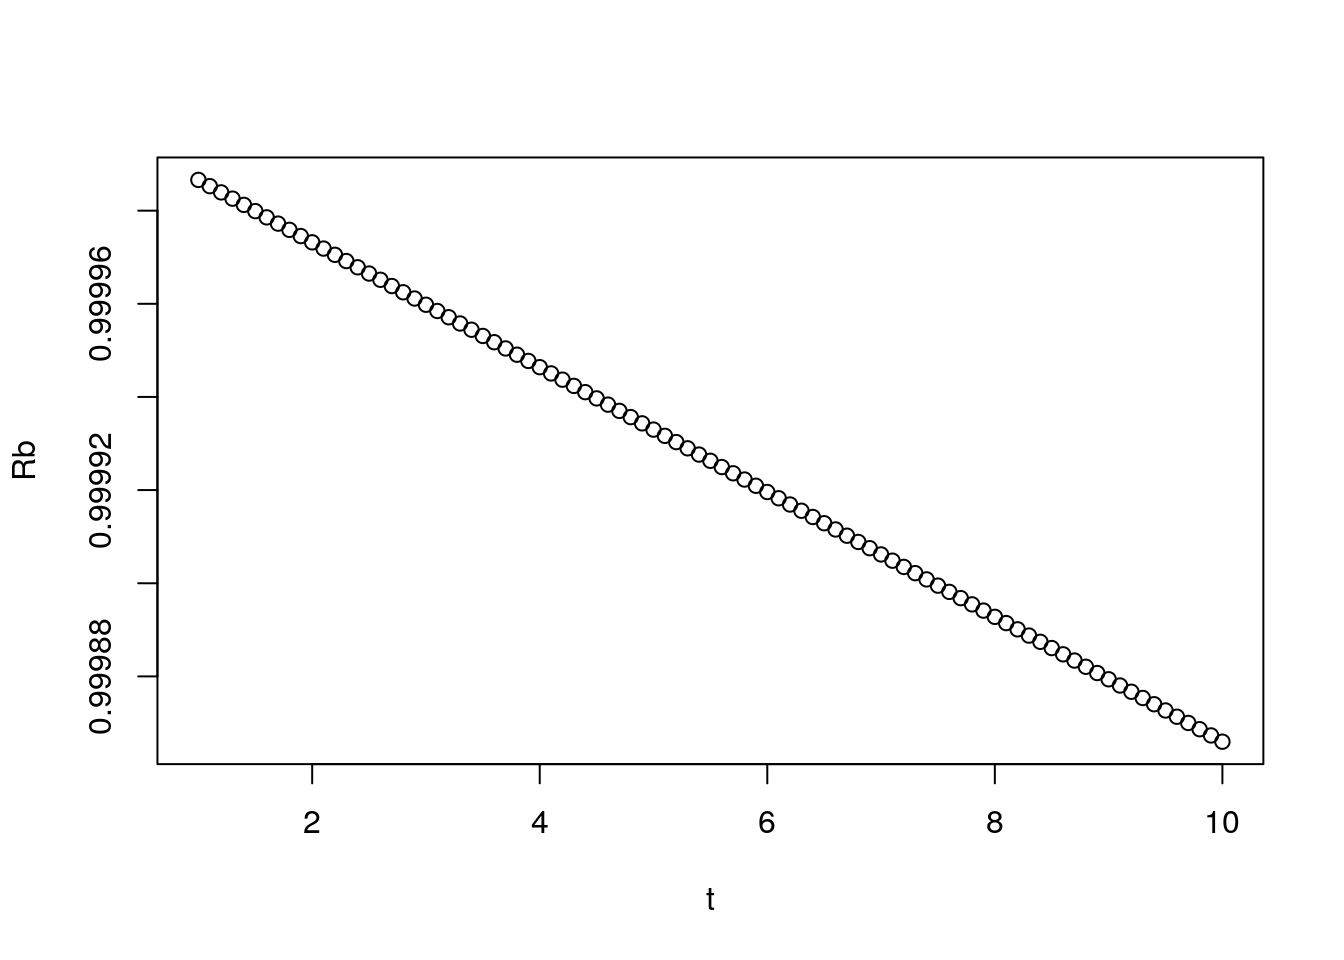
\includegraphics{livro_files/figure-latex/unnamed-chunk-10-1.pdf}

\chapter{Aplicações}\label{aplicauxe7uxf5es}

Neste capítulo apresentaremos alguns exemplos de aplicações de R.

\section{Exemplo 1}\label{exemplo-1}

\subsection{Carregamento de dados}\label{carregamento-de-dados}

\begin{Shaded}
\begin{Highlighting}[]
\NormalTok{########################################################################################}
\CommentTok{#1-Carregamento de dados}
\CommentTok{#1.1-Dados do Covid19  }
\CommentTok{# referencia(22-06-2020) - (https://data.brasil.io/dataset/covid19/_meta/list.html)}

\KeywordTok{library}\NormalTok{(readr)}

\NormalTok{caso <-}\StringTok{ }\KeywordTok{read_csv}\NormalTok{(}\StringTok{"data/caso.csv"}\NormalTok{)}
\end{Highlighting}
\end{Shaded}

\begin{verbatim}
## Parsed with column specification:
## cols(
##   date = col_date(format = ""),
##   state = col_character(),
##   city = col_character(),
##   place_type = col_character(),
##   confirmed = col_double(),
##   deaths = col_double(),
##   order_for_place = col_double(),
##   is_last = col_logical(),
##   estimated_population_2019 = col_double(),
##   city_ibge_code = col_double(),
##   confirmed_per_100k_inhabitants = col_double(),
##   death_rate = col_double()
## )
\end{verbatim}

\section{Análise de dados}\label{anuxe1lise-de-dados}

\subsection{Análise Exploratória}\label{anuxe1lise-exploratuxf3ria}

\begin{verbatim}
## Parsed with column specification:
## cols(
##   regiao = col_character(),
##   estado = col_character(),
##   municipio = col_logical(),
##   coduf = col_double(),
##   codmun = col_logical(),
##   codRegiaoSaude = col_logical(),
##   nomeRegiaoSaude = col_logical(),
##   data = col_character(),
##   semanaEpi = col_double(),
##   populacaoTCU2019 = col_double(),
##   casosAcumulado = col_double(),
##   casosNovos = col_double(),
##   obitosAcumulado = col_double(),
##   obitosNovos = col_double(),
##   Recuperadosnovos = col_double(),
##   emAcompanhamentoNovos = col_double()
## )
\end{verbatim}

\begin{verbatim}
## Warning: 1727211 parsing failures.
##  row    col           expected actual                                     file
## 3305 codmun 1/0/T/F/TRUE/FALSE 110000 'data/HIST_PAINEL_COVIDBR_21jun2020.csv'
## 3306 codmun 1/0/T/F/TRUE/FALSE 110000 'data/HIST_PAINEL_COVIDBR_21jun2020.csv'
## 3307 codmun 1/0/T/F/TRUE/FALSE 110000 'data/HIST_PAINEL_COVIDBR_21jun2020.csv'
## 3308 codmun 1/0/T/F/TRUE/FALSE 110000 'data/HIST_PAINEL_COVIDBR_21jun2020.csv'
## 3309 codmun 1/0/T/F/TRUE/FALSE 110000 'data/HIST_PAINEL_COVIDBR_21jun2020.csv'
## .... ...... .................. ...... ........................................
## See problems(...) for more details.
\end{verbatim}

\begin{verbatim}
## `summarise()` ungrouping output (override with `.groups` argument)
\end{verbatim}

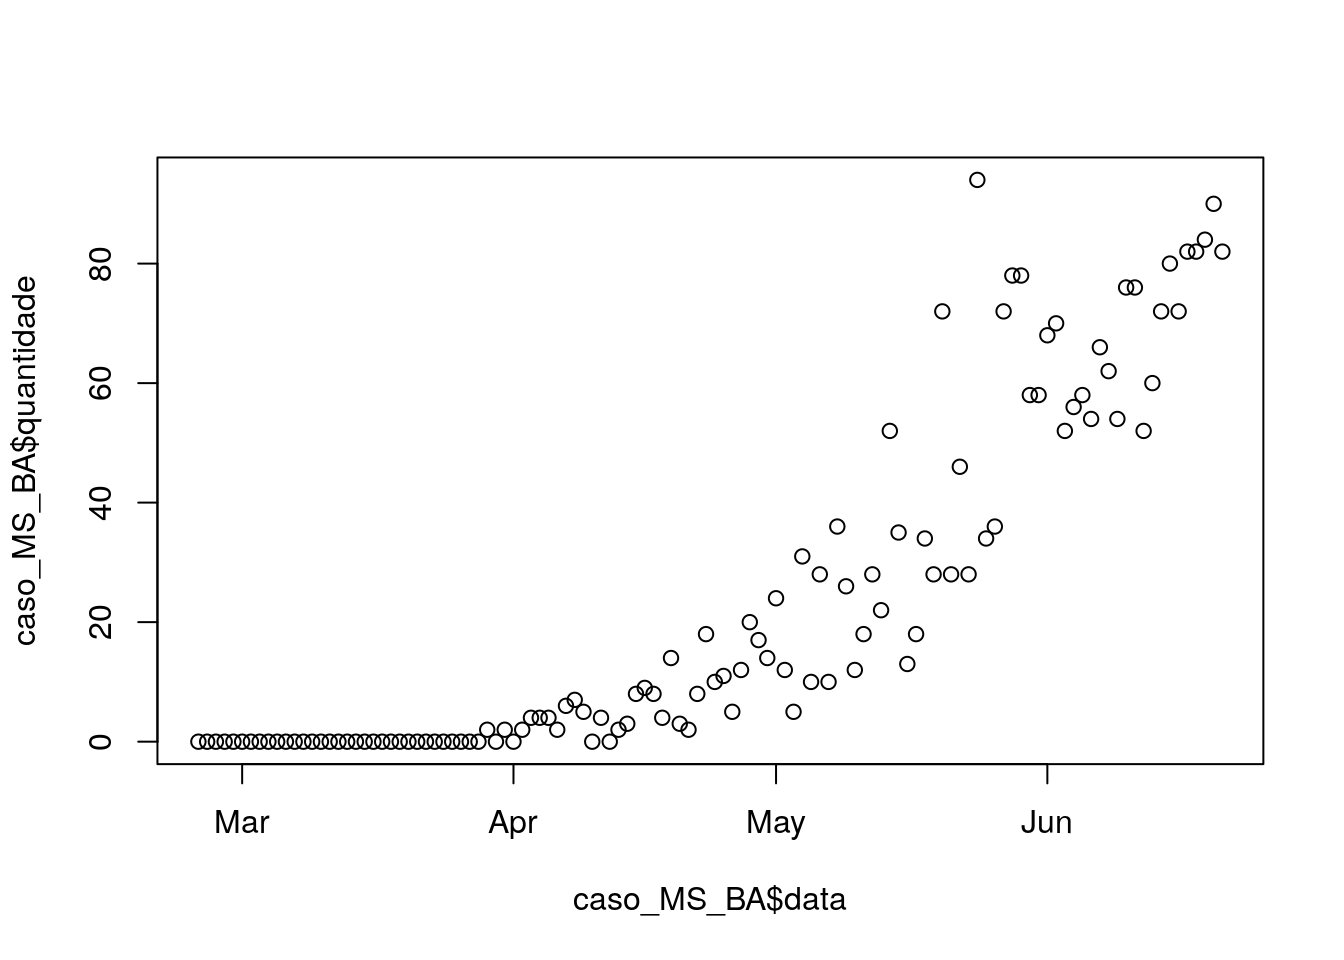
\includegraphics{livro_files/figure-latex/unnamed-chunk-12-1.pdf}

\begin{verbatim}
## `summarise()` ungrouping output (override with `.groups` argument)
\end{verbatim}

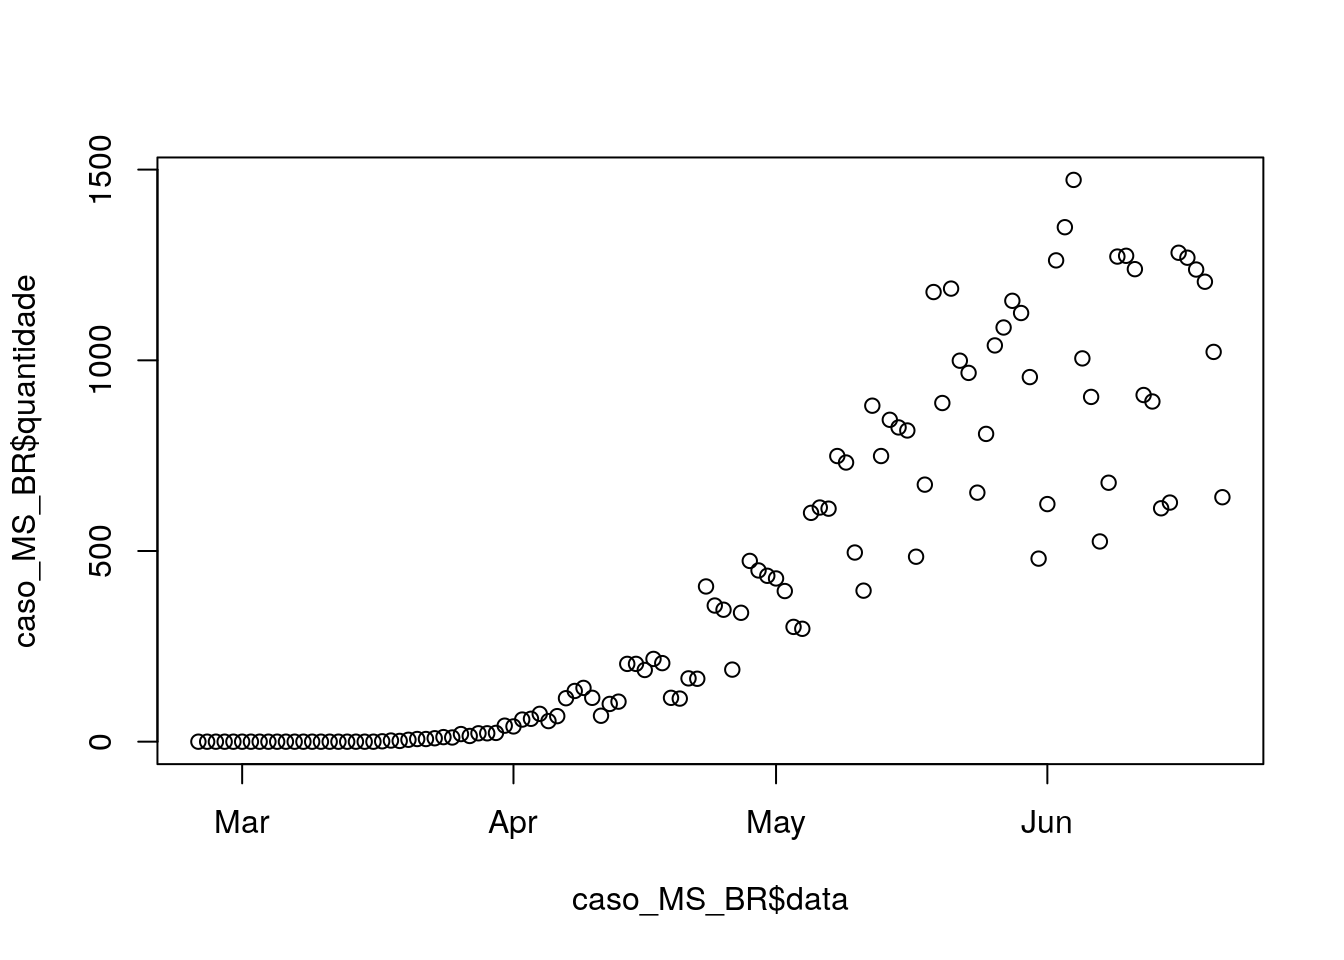
\includegraphics{livro_files/figure-latex/unnamed-chunk-12-2.pdf}
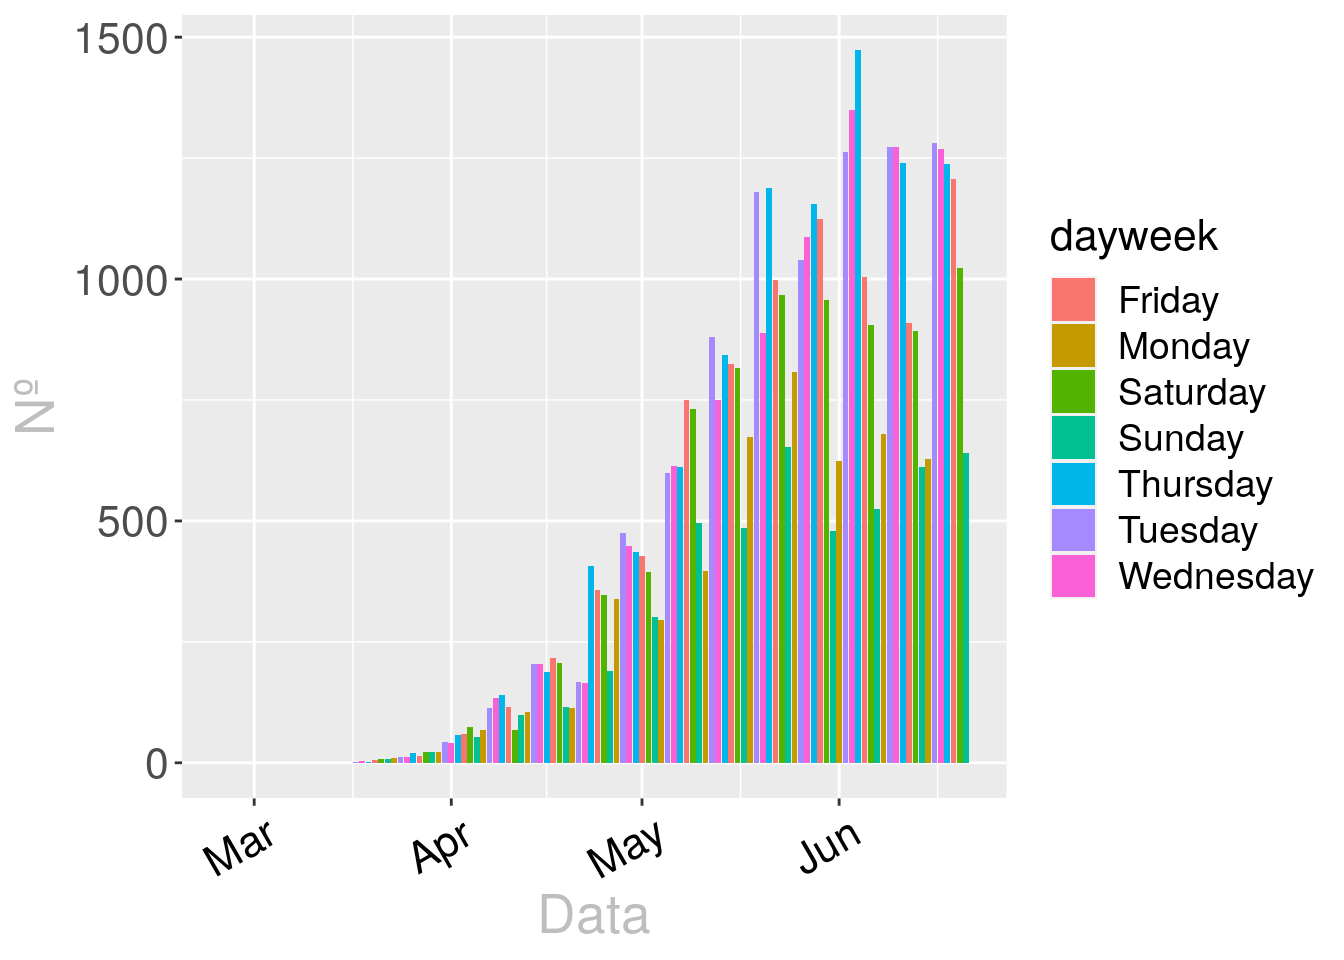
\includegraphics{livro_files/figure-latex/unnamed-chunk-12-3.pdf}

\chapter{Recomendações finais}\label{recomendauxe7uxf5es-finais}

A principal sugestão para o contexto desse projeto é que haja um
controle para que duas pessoas não trabalhem no mesmo capítulo durante o
mesmo período num diretório de github, essa prática pode ampliar demais
o trabalho de quem gerencia as pastas do github. Embora haja os recursos
de Brunch, se duas ou mais pessoas trabalham num mesmo cápitulo pode se
tornar um pouco confuso o merge de capítulos.

\section{O site principal do
Bookdown}\label{o-site-principal-do-bookdown}

\url(\url{https://bookdown.org/})

\section{Reportagem}\label{reportagem}

\url(\url{https://medium.com/@diegousaiuk/how-i-used-hugo-and-blogdown-to-set-up-my-own-website-e32e2eddbf81})

\textbf{Treinar Tidyverse}

Após o treino dos recursos do tidyverse e especialmente o ggplot
apresentados por Ícaro Bernardes, por favor, explorem neste ambinte a
inclusão dos exercícios. Procurar pasta de capacitação disponível no
github \url(\url{https://github.com/cienciadedadosnaep}) . Como
recomendado pelo facilitador Ícaro Bernardes, acessar os documentos
\emph{Cheat Sheet} no site
\url(\url{https://rstudio.com/resources/cheatsheets/}).

\textbf{Tidyverse}

\begin{itemize}
\tightlist
\item
  Tidyverse
\end{itemize}

\textbf{Ggplot}

\begin{itemize}
\tightlist
\item
  ggplot
\end{itemize}

\bibliography{book.bib,packages.bib}

\end{document}
